\subsection{Apply transformation}
\label{subsection:applyTransformation}

\begin{figure}[!h]
\begin{center}
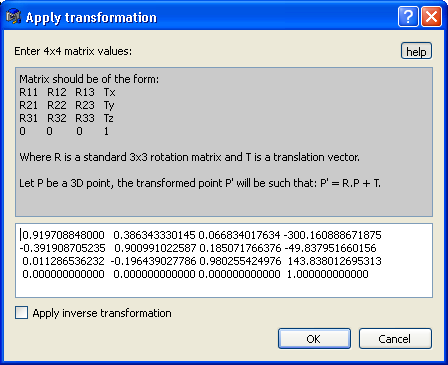
\includegraphics[width=0.5\textwidth]{Partie3_Fonctions/applyTransformation.png}
\caption{\label{fig:applyTransformation}Interface de d�finition d'une transformation 3D (\textit{avec aide affich�e})}
\end{center}
\end{figure}

Cet outil permet � l'utilisateur de sp�cifier une transformation 3D (matrice $4\times4$ compos�e d'une matrice de rotation dans la partie sup�rieure � gauche et d'un vecteur translation dans la partie sup�rieure de la derni�re colonne). Cette transformation (ou son inverse si la case � cocher \textit{Apply inverse transformation} est activ�e) peut alors �tre appliqu�e aux entit�es s�lectionn�es.\\
\par
Remarques :
\begin{itemize}
\item une aide peut-�tre affich�e en appuyant sur le bouton en haut � gauche (voir figure~\ref{fig:applyTransformation}).
\item apr�s une transformation manuelle (voir section~\ref{subsection:graphicalTransformation}) ou un recalage de type ICP (voir section~\ref{subsection:register}) CloudCompare affiche dans la console la transformation appliqu�e aux entit�s. Cette transformation peut-�tre s�lectionn�e dans la console et r�cup�r�e - en \textit{copiant} le texte avec CTRL+C - puis \textit{coll�e} - CRTL+V - dans l'outil (attention, il faut faire attention aux premiers caract�res du texte coll� qui correspondent � l'heure du message et qui doivent donc �tre supprimm�s avant d'appliquer la transformation !). Ceci permet notamment soit d'annuler une transformation (en appliquant la transformation inverse) ou alors d'appliquer la m�me transformation � une autre entit�e apr�s un recalage (on peut en effet vouloir segmenter/nettoyer un nuage avant d'appliquer l'algorithme ICP - pour obtenir un meilleur recalage - puis appliquer la transformation obtenue au nuage d'origine).\\
\end{itemize}

